% ============================================================================
% COLM 2026 Workshop on Efficient Reasoning submission
% "Reasoning Tokens Buy Competence, Not Compliance"
%
% SUBMISSION NOTE: swap this preamble for the official COLM 2026 style
% (\usepackage{colm2026_conference}) before OpenReview upload — body is
% template-agnostic. 4-10 pages main text allowed; this draft ~6-7.
% Numbers auto-generated: scripts/make_workshop_assets.py + make_paper_macros.py.
% ============================================================================
\documentclass[11pt]{article}
\usepackage[margin=1in]{geometry}
\usepackage{amsmath,amssymb}
\usepackage{booktabs}
\usepackage{graphicx}
\usepackage[hidelinks]{hyperref}
\usepackage{microtype}
\graphicspath{{generated/}}
% AUTO-GENERATED by scripts/make_workshop_assets.py
\newcommand{\WMeanRev}{74.2}
\newcommand{\WBandMin}{63}
\newcommand{\WBandMax}{81}
\newcommand{\WNCols}{18}
\newcommand{\WGptFiveB}{10}
\newcommand{\WGptFiveC}{0}
\newcommand{\WAggB}{401}
\newcommand{\WAggC}{6}
\newcommand{\WGptFiveDefaultCost}{8.3}
\newcommand{\WGptFiveDefaultN}{121}
\newcommand{\WGptFiveDefaultTrunc}{121}
\newcommand{\WGptFiveLowCost}{7.4}
\newcommand{\WGptFiveLowN}{248}
\newcommand{\WGptFiveLowTrunc}{144}
\newcommand{\WGptFiveMinCost}{1.6}
\newcommand{\WPooledRev}{75.9}
\newcommand{\WTrendZ}{1.40}
\newcommand{\WTrendP}{0.16}

% AUTO-GENERATED by scripts/make_paper_macros.py — do not edit
\newcommand{\AggB}{401}
\newcommand{\AggC}{6}
\newcommand{\AggRatio}{67}
\newcommand{\BandMin}{63}
\newcommand{\BandMax}{81}
\newcommand{\BandMean}{74.2}
\newcommand{\BandN}{18}
\newcommand{\CompetenceSpanX}{792}
\newcommand{\GemmaOrH}{51}
\newcommand{\GemmaP}{3e-49}
\newcommand{\CtlGemmaRev}{85}
\newcommand{\CtlGemmaSci}{89}
\newcommand{\CtlDsRev}{97}
\newcommand{\CtlDsSci}{90}
\newcommand{\RetestMean}{86.2}
\newcommand{\RetestSD}{4.7}
\newcommand{\RetestUnanimity}{40}
\newcommand{\RetestK}{5}
\newcommand{\TvPass}{125/125}
\newcommand{\NInstances}{1000}
\newcommand{\NPhysics}{125}
\newcommand{\NFamilies}{7}
\newcommand{\NColumns}{18}


\title{\textbf{Reasoning Tokens Buy Competence, Not Compliance}\\[3pt]
\large What test-time compute does --- and does not --- purchase,\\
measured with a sign-exact oracle}
\author{Mayank Ravishankara}
\date{}

\begin{document}
\maketitle

\begin{abstract}
Test-time reasoning is usually evaluated on one axis: does more thinking buy
more accuracy per token? We add the axis that efficiency work has ignored ---
\emph{compliance}: when an explicit instruction opposes a convention the model
absorbed in training, do reasoning tokens help the instruction win? Using
CircuChain~v2, a circuit-analysis probe whose answers are verifiable to the
sign by four independent solvers, we measure both axes across
\WNCols{} model configurations from \NFamilies{} families. Three findings.
(1)~\textbf{Reasoning buys competence only}: toggling the same weights between
reasoning and non-reasoning modes at five scales (Qwen3 1.7B--32B) raises
magnitude accuracy up to $3\times$ while reversion to the trained convention
stays flat --- \WBandMin--\WBandMax\% (mean \WMeanRev\%) everywhere, a band
that also contains GPT-5, Gemma-4, GPT-OSS-120B, and DeepSeek-V3 across a
\CompetenceSpanX$\times$ competence range.
(2)~\textbf{The GPT-5 reasoning-effort ladder dissociates the axes}: at
\texttt{minimal} effort it answers from the prior --- cheaply and wrongly; at
\texttt{low} effort it solves sign-trap circuits to nine decimals yet still
reports the trained frame $\sim$71\% of the time; at \texttt{default} effort
reasoning consumes the entire token budget and \emph{zero} of 119 requests
return an answer at the highest cost per instance.
(3)~\textbf{Unbounded rumination is a real cost}: below the competence
threshold, reasoning modes burn the full 16k budget on 73--77\% of problems
without converging. Across all models, flipping one convention instruction
breaks \WAggB{} previously-solved problems and fixes \WAggC{}. Efficiency
evaluations that report accuracy-per-token implicitly assume compute
purchases controllability; our oracle-verified evidence says it does not.
We release the generator, oracle, and harness; total study cost was under
\$100.
\end{abstract}

% ----------------------------------------------------------------------------
\section{Introduction}

The efficient-reasoning agenda optimizes a ratio: capability delivered per
unit of test-time compute. Its numerator is almost always \emph{accuracy}.
This paper measures a second numerator that practitioners implicitly assume
comes bundled with the first: \emph{compliance} --- whether the model does the
task \emph{the way it was told to}, when the instruction opposes a strong
prior from training.

The distinction matters exactly when models are deployed against
specifications: house styles, legacy code conventions, discipline-specific
sign disciplines, safety policies that differ from common practice. If
reasoning tokens buy accuracy but not obedience, then (i) scaling test-time
compute does not close the steerability gap, (ii) efficiency benchmarks that
score only correctness will not see the gap at any budget, and (iii) budget
tuning (effort levels, early stopping, distillation) can be evaluated on a
false frontier.

Measuring this cleanly requires a task where compliance is \emph{objectively
decidable at the precision the instruction affects}. We use linear DC circuit
analysis: the answer is exact; a sign convention (e.g.\ the direction mesh
currents are defined) changes only the \emph{reporting frame}, never the
physics; and the textbook prior is overwhelmingly one-sided (clockwise).
CircuChain~v2 poses \NInstances{} instances --- \NPhysics{}
four-way-verified physics configurations $\times$ \{default contract, three
single-factor convention flips\} $\times$ \{mesh, nodal\} --- and grades
deterministically against an oracle validated independently of the transform
code (\TvPass{} configurations). Within-physics matched pairs give exact
McNemar tests: the causal effect of one changed sentence.

\paragraph{Contributions for this workshop.}
(1)~A compute-vs-compliance measurement: the reasoning toggle held at fixed
weights across five scales, plus the GPT-5 effort ladder, with per-instance
dollar costs. (2)~The negative result: no reasoning budget, at any scale or
effort, reduces reversion to the trained convention
(\WBandMin--\WBandMax\% everywhere). (3)~An efficiency pathology inventory
measured with an exact oracle: prior-driven fast-wrong answers at low effort,
budget-consuming rumination at high effort, and 100\%-truncation regimes
where the most expensive configuration returns nothing. (4)~A released,
seeded, LLM-free instrument cheap enough for budget-sweep studies
(full panel $<\$100$).

% ----------------------------------------------------------------------------
\section{Instrument in brief}
\label{sec:instrument}

CircuChain v2 extends our published probe \cite{ravishankara2026circuchain}.
\NPhysics{} physics configurations across seven linear-DC topologies are
accepted only when two independent hand-derived solvers, an exact
rational-arithmetic MNA solver, and NGSPICE agree on every quantity; sign
traps and controls are balanced $\sim$1:1 by code predicates. Each physics is
posed under the textbook-default contract and three single-factor flips ---
mesh direction \texttt{cw}$\to$\texttt{ccw}, passive$\to$active sign,
reference node bottom$\to$top --- in both mesh (KVL) and nodal (KCL) methods.
Expected answers in every frame are validated independently of the transform
code, including a \emph{physically re-grounded} SPICE realization of the
reference-node flip. Grading is deterministic (structured answer-line parser;
magnitude at 2\%; sign compliance in the \emph{instructed} frame; truncation
recorded as an outcome). Decoding: temperature 0.6, top-$p$ 0.95, 16{,}384
completion budget for reasoning modes, 4{,}096 otherwise. Variables whose
sign differs between instructed and default frames are \emph{diagnostic};
reversion is measured on those, given correct magnitude.

% ----------------------------------------------------------------------------
\section{Reasoning raises competence, never compliance}
\label{sec:toggle}

Qwen3's native \texttt{/think} toggle switches reasoning on/off with weights,
prompt, serving stack, and decoding policy fixed --- the cleanest possible
compute contrast. Table~\ref{tab:c1} shows the five-scale result: magnitude
competence rises with reasoning at every scale (e.g.\ 14B: $2.8\%\to9.3\%$),
while reversion to the clockwise frame among magnitude-correct diagnostic
variables never moves outside the band (68--81\%, all CIs overlapping).
Reasoning tokens purchase physics, not obedience.

\begin{table}[t]
\centering\small
\begin{tabular}{lcccc}
\toprule
 & \multicolumn{2}{c}{No-think} & \multicolumn{2}{c}{Think (16k budget)}\\
Scale & Mag.\ correct & Reversion ($n$) & Mag.\ correct & Reversion ($n$)\\
\midrule
% AUTO-GENERATED — do not edit
1.7b & 0.2\% & 71\% (24) & 2.4\% & 72\% (69) \\
4b & 0.7\% & 68\% (37) & 5.0\% & 70\% (47) \\
8b & 1.2\% & 70\% (61) & 2.1\% & 81\% (31) \\
14b & 2.8\% & 75\% (91) & 9.3\% & 78\% (91) \\
32b & 5.1\% & 77\% (102) & 8.6\% & 76\% (62) \\

\bottomrule
\end{tabular}
\caption{The reasoning toggle at fixed weights (Qwen3 ladder). Reversion =
share of magnitude-correct sign-diagnostic variables reported in the trained
clockwise frame despite the counter-clockwise instruction.}
\label{tab:c1}
\end{table}

\paragraph{The cost side.}
Table~\ref{tab:trunc} shows what the reasoning budget buys at the small end:
below the competence threshold, think modes ruminate to the full 16k budget
on most problems (truncations: 727--769 of 1000 at 4B--32B) --- genuine
self-correction spirals that never converge. This is paid-for compute
delivering neither competence nor compliance; larger budgets shift the wall
rather than remove it.

\begin{table}[t]
\centering\small
\begin{tabular}{lcccc}
\toprule
 & \multicolumn{2}{c}{No-think} & \multicolumn{2}{c}{Think}\\
Scale & Mag.\ correct & Truncated & Mag.\ correct & Truncated\\
\midrule
% AUTO-GENERATED
1.7b & 0.2\% & 30 & 2.4\% & 164 \\
4b & 0.7\% & 1 & 5.0\% & 742 \\
8b & 1.2\% & 1 & 2.1\% & 732 \\
14b & 2.8\% & 0 & 9.3\% & 727 \\
32b & 5.1\% & 4 & 8.6\% & 769 \\

\bottomrule
\end{tabular}
\caption{Rumination economics on the Qwen3 ladder (of 1000 instances).
Reasoning modes burn the full completion budget on most instances while
magnitude competence stays under 10\%.}
\label{tab:trunc}
\end{table}

% ----------------------------------------------------------------------------
\section{The GPT-5 effort ladder: three budgets, three failure modes}
\label{sec:gpt5}

GPT-5's reasoning-effort control exposes the compute--behavior trade
directly on one frontier model (Figure~\ref{fig:gpt5}):

\textbf{\texttt{minimal}} ($\approx$\WGptFiveMinCost¢/instance): reasoning
tokens $=0$; the model answers instantly --- \emph{from the prior} --- and
gets the physics wrong on our probe.
\textbf{\texttt{low}} ($\approx$\WGptFiveLowCost¢): on a 248-instance run it
solves sign-trap circuits exactly when it completes (magnitude-correct 32.7\%
overall, best of any reasoning configuration we ran under this budget) ---
and still reports the trained frame on 70.6\% of magnitude-correct
diagnostic variables; the paired ccw flip breaks \WGptFiveB{} problems and
fixes \WGptFiveC.
\textbf{\texttt{default}} ($\approx$\WGptFiveDefaultCost¢, the most
expensive): hidden reasoning consumed the \emph{entire} 8{,}192-token budget
on 119 of 119 requests --- zero answers returned, at the highest per-instance
cost.

The ladder dissociates the axes cleanly: compliance is not purchasable at any
of the three budgets, competence is purchasable at exactly one of them, and
the default configuration purchases nothing. For efficiency work, the
\texttt{default} row is the cautionary tale: without budget-aware evaluation,
a deployment can pay maximum cost for a 0\% answer rate.

\begin{figure}[t]
\centering
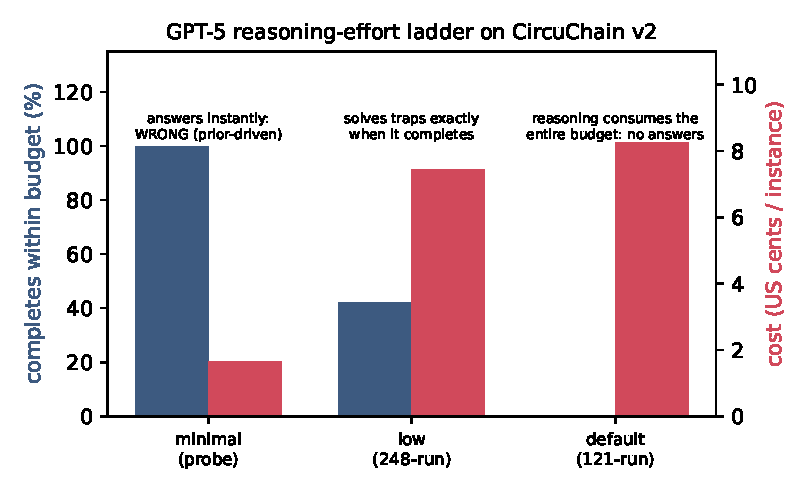
\includegraphics[width=0.72\linewidth]{fig_gpt5_effort.pdf}
\caption{GPT-5 reasoning-effort ladder on CircuChain v2: completion-within-
budget rate (left axis) and measured cost per instance (right axis).
\texttt{minimal} completes always but answers from the prior (wrong);
\texttt{low} is the only configuration that buys competence; \texttt{default}
spends the most and returns nothing. Compliance with the counter-normative
convention is $\sim$29\% regardless.}
\label{fig:gpt5}
\end{figure}

% ----------------------------------------------------------------------------
\section{The invariant that compute never moves}
\label{sec:invariant}

Figure~\ref{fig:inv} is the study's central object: reversion to the trained
clockwise frame among magnitude-correct diagnostic variables, for every panel
configuration with $n\ge20$, against task competence on a log axis. The band
is \WBandMin--\WBandMax\% (mean \WMeanRev\%) across \WNCols{} configurations
spanning \NFamilies{} families, $\sim$\CompetenceSpanX$\times$ in
competence, two serving stacks, and both reasoning modes. Aggregated over all
models, the within-physics paired flip breaks \WAggB{} solved problems and
fixes \WAggC{} (\AggRatio:1) --- reversion, not noise.

Three controls establish that this is convention-specific reversion rather
than generic instruction decay: the same models follow matched
\emph{non-convention} unusual instructions (reversed answer order,
scientific notation) at \CtlGemmaRev--\CtlDsRev\%; GPT-5 and Gemma obey the
\emph{other two} convention factors while disobeying mesh direction; and the
effect is equal on trap and control physics. The reversion also persists
under nodal solving, where loop orientation never enters the derivation ---
it is a property of the \emph{reporting frame}, not the procedure. Resampling
(k=\RetestK) shows a stable rate (SD \RetestSD{}pp) over stochastic items:
a biased coin, $\sim$4:1 toward the trained frame, at every budget.

\begin{figure}[t]
\centering
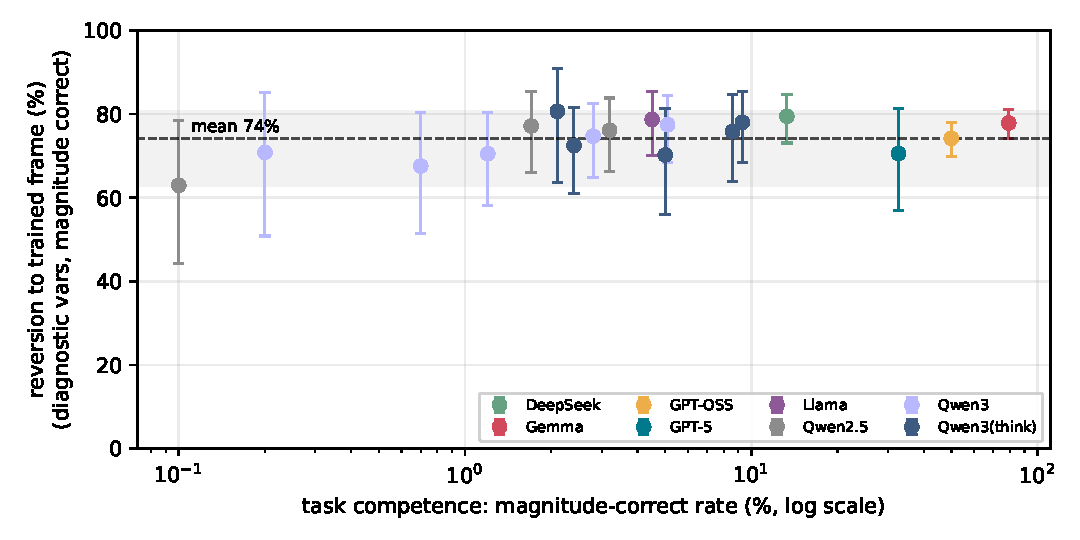
\includegraphics[width=\linewidth]{fig_invariance.pdf}
\caption{Reversion to the clockwise prior is invariant to competence, scale,
family, serving stack, and reasoning mode. Each point is one panel
configuration (Wilson 95\% CIs; $n\ge20$ diagnostic variables); shaded band
= observed range \WBandMin--\WBandMax\%.}
\label{fig:inv}
\end{figure}

% ----------------------------------------------------------------------------
\section{Implications for efficient reasoning}
\label{sec:implications}

\textbf{1. Put compliance in the efficiency numerator.} Accuracy-per-token
frontiers implicitly assume behavior is purchasable with compute. Measured
with an exact oracle, it is not: the compliance curve is flat in compute.
Efficiency evaluations --- especially of effort controls, early-stopping, and
distillation --- should report \emph{constraint adherence per token}
alongside accuracy per token, using probes whose compliance is mechanically
decidable (ours is released and costs cents per thousand instances).

\textbf{2. Budget-aware evaluation is not optional.} The most expensive
GPT-5 configuration returned zero answers; small reasoning models burn full
budgets on 73--77\% of instances without converging. Truncation must be a
first-class reported outcome, or efficiency comparisons silently reward
configurations that never finish.

\textbf{3. Effort controls are behavioral, not just economic.} Moving GPT-5
from \texttt{minimal} to \texttt{low} switches it from prior-recitation to
genuine derivation --- a qualitative regime change purchased with tokens; more
tokens past that point purchase nothing measurable. Efficiency work that
tunes effort levels is implicitly selecting \emph{which} failure mode ships.

\textbf{4. Distillation and steering research have a concrete target.} The
frame choice is made outside the reasoning trace (it survives nodal solving
and every budget), and it is sampled ($\sim$4:1) rather than committed. A
cheap deterministic frame-checking/repair layer recovers more reliability per
dollar than any reasoning budget we measured.

% ----------------------------------------------------------------------------
\section{Limitations}
One domain (linear DC circuits); a second convention domain (handedness /
cross products) is in progress. Whole-problem effects rest on the few models
competent at multi-loop circuits (itself an efficiency datum: 70B-class
instruct models sit under 14\% magnitude-correct); variable-level results
cover the full panel. GPT-5 was run at 248 instances under a bounded budget;
its numbers are conservative. Single-sample decoding for most columns is
mitigated by the resampling study and the cross-column invariance.

\section*{Reproducibility}
Seeded byte-reproducible generator (\NPhysics{} physics), four-way oracle,
independent transform validation (\TvPass), deterministic grading, full
serving provenance per response, canary-stamped evaluation subset; code and
harness released. Total API cost $<\$100$; local runs on one Apple M5 Max.

\begin{thebibliography}{9}\small
\bibitem{ravishankara2026circuchain}
M.~Ravishankara. CircuChain: Disentangling competence and compliance in LLM
circuit analysis. In \emph{Proc.\ IEEE SoutheastCon}, 2026. arXiv:2602.15037.

\bibitem{zhang2025inverseifeval}
Q.~Zhang, X.~Lei, R.~Miao, et al.
Inverse IFEval: Can LLMs unlearn stubborn training conventions to follow real
instructions? arXiv:2509.04292, 2025.

\bibitem{wu2024reasoning}
Z.~Wu, L.~Qiu, A.~Ross, E.~Aky\"urek, B.~Chen, B.~Wang, N.~Kim, J.~Andreas,
Y.~Kim. Reasoning or reciting? Exploring the capabilities and limitations of
language models through counterfactual tasks. In \emph{NAACL}, 2024.

\bibitem{zhou2023ifeval}
J.~Zhou, T.~Lu, S.~Mishra, S.~Brahma, S.~Basu, Y.~Luan, D.~Zhou, L.~Hou.
Instruction-following evaluation for large language models.
arXiv:2311.07911, 2023.

\bibitem{snell2024scaling}
C.~Snell, J.~Lee, K.~Xu, A.~Kumar. Scaling LLM test-time compute optimally
can be more effective than scaling model parameters. arXiv:2408.03314, 2024.

\bibitem{chen2024overthinking}
X.~Chen et al. Do NOT think that much for 2+3=? On the overthinking of
o1-like LLMs. arXiv:2412.21187, 2024.
\end{thebibliography}

\end{document}
